\documentclass[
        a4paper,
        10pt,
        parskip = full,    % Layout with zero \parident and non-zero \parskip
    ]{scrartcl}
% \usepackage[utf8]{inputenc}

\usepackage[top=2cm, bottom=2.5cm, left=2.5cm, right=2.5cm]{geometry}
\usepackage[
        colorlinks = true,    % Disable drawing boxes around links.
        linkcolor = black,    % Sets the color of links to black.
    ]{hyperref}
\usepackage{amsmath}
\usepackage{graphicx}
\usepackage{subfig}
\usepackage{float}

\begin{document}

\textbf{\large{Laboratory - Deep Learning Lab, WS 2018/2019 - Exercise 4}}

\textbf{\large{Submitted by:\\
\\
Amadeus Hovekamp,\\
mail@amadeus-hovekamp.de,\\
Matr. no: 4603934\\
\\
Hans N\"ubel,\\
hans.nuebel@rwth-aachen.de,\\
Matr. no: 4514598}}

The repository with the source code can be found under the following link:\\
\href{https://github.com/Schokokugel/RoboticsLab}
     {https://github.com/Schokokugel/RoboticsLab}


\section{Getting Set Up}

As the set up for this exercise was the same as for the last exercise, there were no issues here.

\section{Reinforcement Learning: Deep Q-Networks}

\subsection{CartPole}

All in all the implementation of the DQN went well, the provided components
helped to implement it. We implemented some additional features that helped us
training the network and generating the required data for writing the report.


The first runs were not successfull due to the small default learning
rate of 0.0001. Changing the learning rate to 0.001 lead to good results,
which can be seen in the following figures \ref{CartPoleTrainEvalReward}
and \ref{CartPoleTestReward}.


The total run had a length of 500 episodes, the reward for each episode is
displayed by the black dots in figure~\ref{CartPoleTrainEvalReward}. The orange dots
show the evaluation reward after every tenth episode, averaged over 5 evaluation
runs using only deterministic actions.

It took the agent about 120 episodes to learn how to prevent the pole from tilting
but it still drove off to the side quickly. After 180 it was sometimes able to
balance the pole for the complete episode consisting of 1000 steps. 40 episodes
later it managed to do so consistently. Somewhat suprisingly it $unlearned$ how to balance the pole after 60 episodes later. This could be due to more and more
of the same states (the pole is almost upright, neither cart or the pole move much)
filling up the replay buffer and thus overfitting the network to highly similar
states. This would also explain the learning-unlearning oszillations later on.
A hint in the source code defined the task as $solved$ when the average reward is
greater than or equal to 195.0 over 100 consecutive trials, which was reached
after 170 episodes.

Figure~\ref{CartPoleTestReward} shows the test rewards achieved with the trained
networks over 15 episodes, once where the network was trained until it is
considered as solved, and once after training for the full run of 500 episodes.
It is visible, that the longer trained network achieved better results.

\begin{figure}[H]
  \begin{center}
    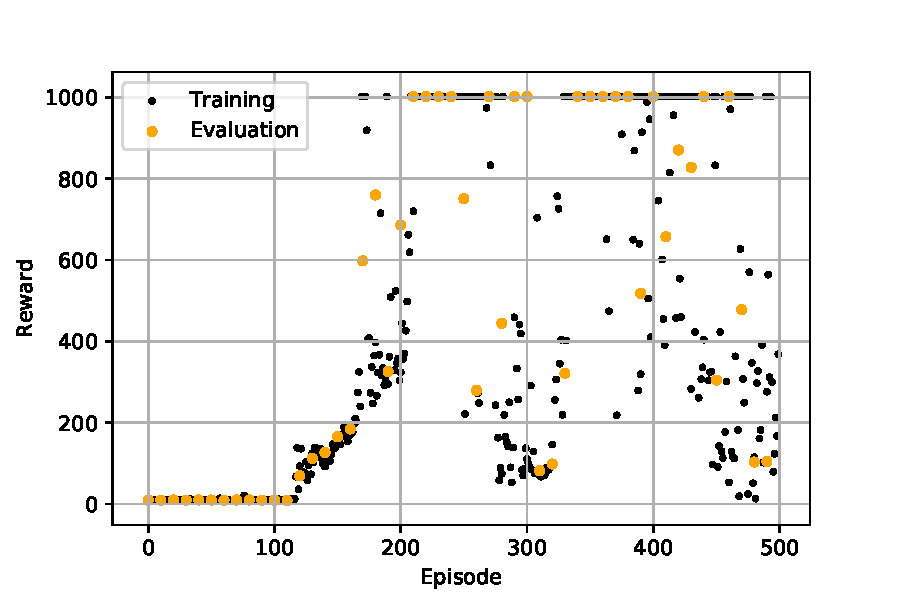
\includegraphics{./images/CartPole-v0/tb_train_eval_reward.pdf}
    \caption{CartPole - Episode Reward during Training}
    \label{CartPoleTrainEvalReward}
  \end{center}
\end{figure}

\begin{figure}[H]
  \begin{center}
    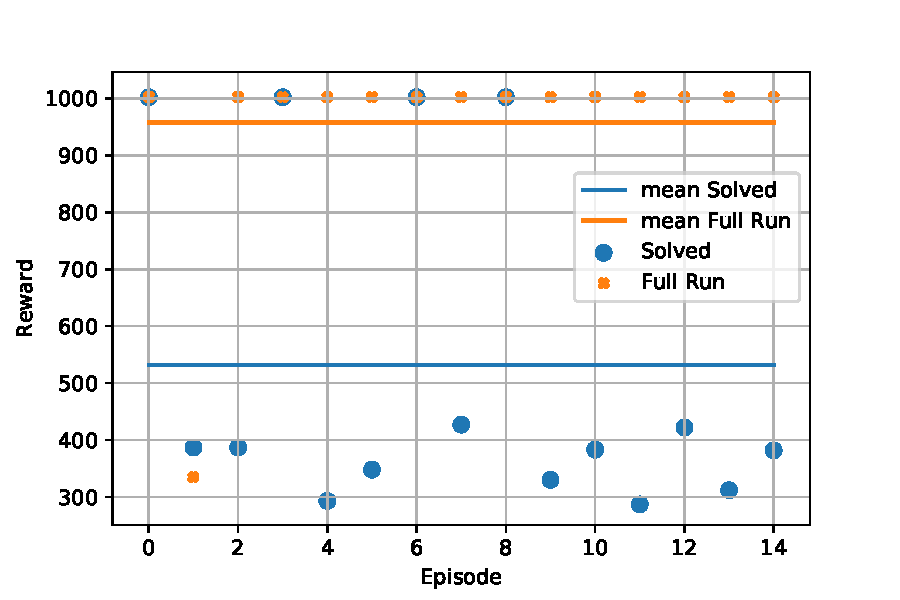
\includegraphics{./images/CartPole-v0/tb_test_reward.pdf}
    \caption{CartPole - Episode Reward for Testing}
    \label{CartPoleTestReward}
  \end{center}
\end{figure}


\subsection{MountainCar}

For the MountainCar environment we used the same setup and network as for the
CartPole environment, leading also to good results, which are displayed in the
figures~\ref{MountainCarTrainEvalReward} and~\ref{MountainCarTestReward}.

\begin{figure}[H]
  \begin{center}
    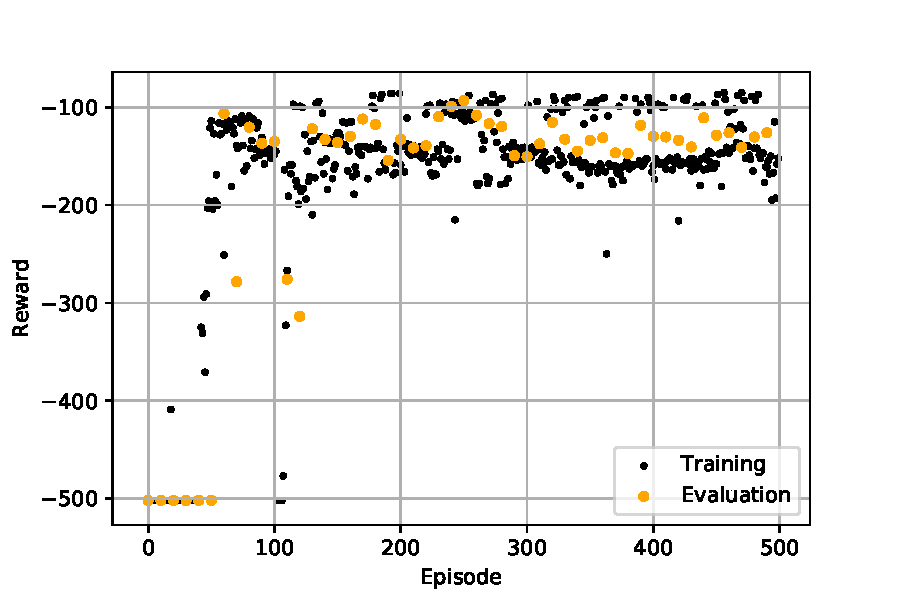
\includegraphics{./images/MountainCar-v0/tb_train_eval_reward.pdf}
    \caption{MountainCar - Episode Reward during Training}
    \label{MountainCarTrainEvalReward}
  \end{center}
\end{figure}

In figure~\ref{MountainCarTrainEvalReward} the training and evaluation rewards
are displayed as in the CartPole environment. Here, already after 60
episodes the network performs good. But later on again an oscillation behavior
can be seen, though the bad performances are not as bad
as some performances of the CartPole. A reason for this difference is probably
that the CartPole is more difficult, consisting of two tasks at the same time
(balancing the pole and not drifting off to the side).

Finally, in figure~\ref{MountainCarTestReward} the test rewards for the
solved model and the full run model are displayed. Here, we have defined solved
as reaching an average score larger than -200 over 100 consecutive runs,
similar to the definition as for the CartPole. In contrast to the CartPole,
Solved scores higher on average. But the Full Run is in turn better when
the starting conditions are favorable for its risky driving style trying to
minimize drives trough the valley.

\begin{figure}[H]
  \begin{center}
    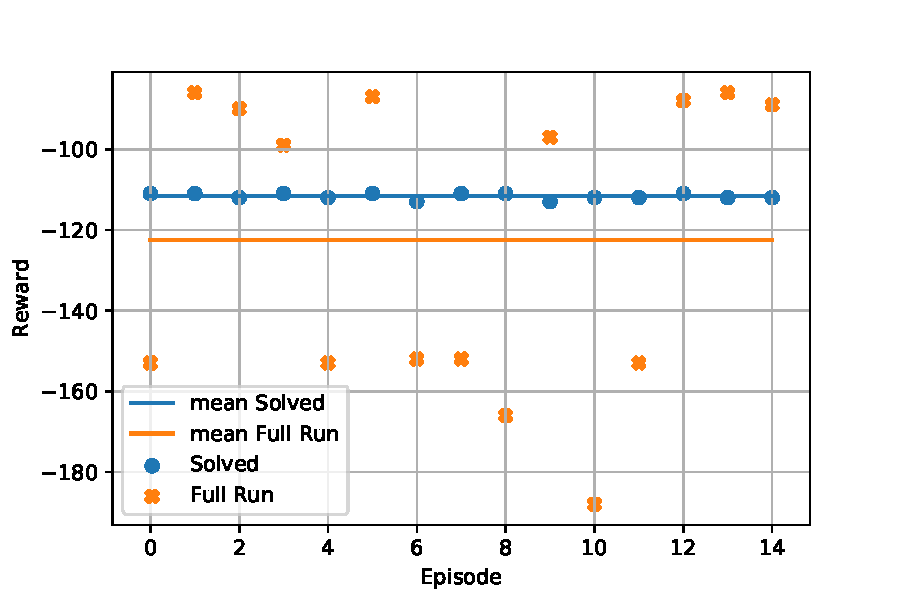
\includegraphics{./images/MountainCar-v0/tb_test_reward.pdf}
    \caption{MountainCar - Episode Reward for Testing}
    \label{MountainCarTestReward}
  \end{center}
\end{figure}


\subsection{CarRacing}

\subsubsection{The network structure}

Our networks from exercise 3 did not perform well and therefore we had to find a
better architecture. So we tried multiple network architectures and trained
them for some time to get a feeling which architecture might work out well. We also
looked at one 98 by 98 images from the game to find how big of a kernel size
should allow the network to recognize certain features like the street contours.

So in the end we used a CCN that consists of two convolution layers (20~filters,
11~kernel size, stride~1), each followed by a max pooling (first: pool\_size~2,
stride 2; second: pool\_size 2, stride 1) and a fully connected layer (128 units).
The input layer size is 98 by 98 by history\_length and output layer contains 5 units.
The history length had a value of 0 or 1. We also experimented with other network
configurations (smaller kernel size / additional fully connected layer, long history
length of 5), but the performance of these networks were worse.

For the training we used a batch size of 64, a learning rate of 0.001 and
skip\_frame set to 1. We did not want to use the skip\_frame option during evalutation
as this would change the problem itself and because we expected that training with a
big skip\_frame would lead to the network performing good in this setting but worse
in the real problem. Therefore we set it to 1, speeding up training and still keeping
training and evaluation settings similar.

\subsubsection{Learning schedule}

For training we defined a learning schedule with different parameters for each run. The values for
each training run can be seen in the following table. As suggested in the exercise, we adapted
the length of the episodes, beginning with 150 steps and increasing it up to 1000 over the 7 training runs.
For the exploration we adapted the percentage of the random actions, beginning with a high value of
20 percent and lowering it too step by step. For values smaller than 5 percent the agent seems to loose
$robustness$, so we increased the value again to 5 in the end. A uniform random action distribution actually
worked out well for us when exluding the STRAIGHT action.

\begin{center}
  \begin{tabular}{ | l | l | l | l | l | l | l | l |}
    \hline
    & \textbf{1st run} & \textbf{2nd run} & \textbf{3rd run} &
    \textbf{4th run} & \textbf{5th run} & \textbf{6th run} & \textbf{7th run} \\ \hline
    \textbf{epsilon}        &  0.2  &  0.15  &  0.1  &  0.05  &  0.04  &  0.03  &  0.05  \\ \hline
    \textbf{max\_timesteps} &  150  &  200   &  300  &  300   &  450   &  700   &  1000  \\ \hline
  \end{tabular}
\end{center}

We experimented with different learning schedules, trying to invoke specific
behaviours in every learning epoch. For example we tried to train the network
to accelerate in the beginning by increasing the portion of random $ACCELERATE$
actions. At first, this works out fine, but later on the agent gets used
to being accelerated randomly and stops to accelerate on its own. For this reason
we also tried a higher rate of random $BRAKE$ actions, leading to more $ACCELERATE$
actions but later on it led to too few $BRAKE$ actions. Therefore we decided to
keep the distribution random actions uniform, except for the $STRAIGHT$ action,
which only remained in the network as it collected several good results thought
out training.

\subsubsection{Results}

Figure \ref{CarRacingTrainEvalReward} shows the training progress of our network
for all 330 episodes. Training the network on a GPU took about 6 to 7 hours.
One can see that the network managed to learn how to drive. When watching the
network train we noticed some milestones: Accelerating, following the
first turn of the road, staying on the road after the road, following the second
turn and so on. These improvements can be seen in the episode reward quite well,
but one has also take into account that the number of timesteps increases step
by step. This also lets the reward go up dramatically. Our network struggled to
drive consistently, unlearning that it has to accelerate in the beginning, chosing
wrong turn actions etc. multiple times during training. This might be a sign that
our network was to small to learn new things while not unlearning previous
knowledge at the same time.

In figure \ref{CarRacingTestReward} the final results of two networks after 8
hours of training on a GPU are shown. One network scored an mean reward of almost
600 over 1000 timesteps and the other only about 350.
The best network managed to achieve about 850 to 870 in many runs clearly showning
its capabilities of driving the car decently. Poor runs also show that it struggled
in two runs early on, not acceleration enough and missing a very tight second
curve. The history did not help to fix the not-accelerating problem.

\begin{figure}
  \begin{center}
    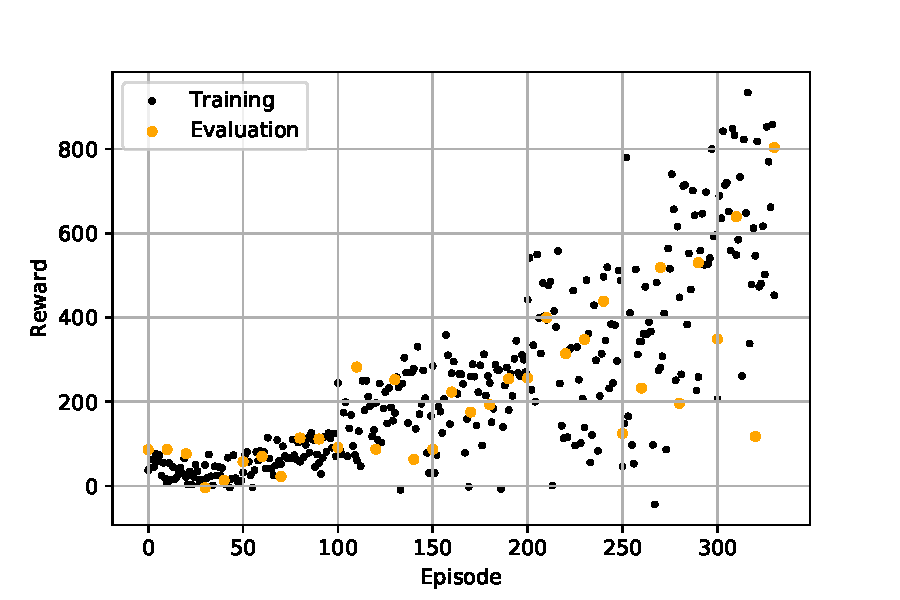
\includegraphics{./images/CarRacing-v0/tb_train_eval_reward.pdf}
    \caption{CarRacing - Episode Reward during Training}
    \label{CarRacingTrainEvalReward}
  \end{center}
\end{figure}


\begin{figure}
  \begin{center}
    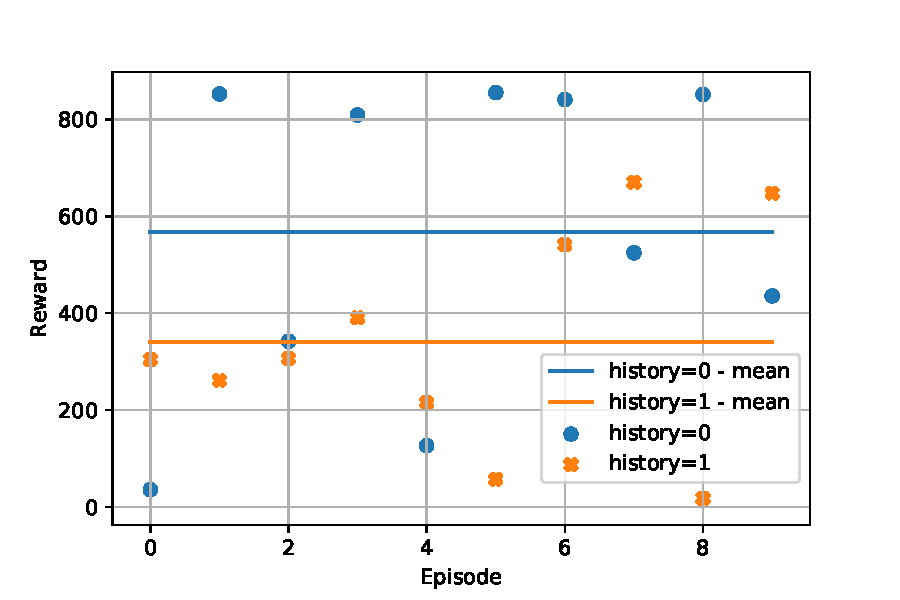
\includegraphics{./images/CarRacing-v0/tb_test_reward.pdf}
    \caption{CarRacing - Episode Reward for Testing}
    \label{CarRacingTestReward}
  \end{center}
\end{figure}


\end{document}
